\documentclass{article}
\usepackage{graphicx,subfig}
\usepackage{graphicx,fancyhdr,amsmath,amssymb,amsthm,subfig,url,hyperref}
\usepackage[margin=1in]{geometry}
\usepackage{subfig}
\usepackage[utf8]{inputenc}
\usepackage{hyperref}
\usepackage{amsmath}
\usepackage{listings}
\usepackage{xcolor} % for customizing colors (optional)
\DeclareUnicodeCharacter{2212}{-}
%\DeclareUnicodeCharacter{2265}{≥}
% \DeclareUnicodeCharacter{2264}{$\leq$}
% \DeclareUnicodeCharacter{2265}{$\beq$}
%----------------------- Macros and Definitions --------------------------
%%% FILL THIS OUT
\lstset{
    language=Matlab, % set language to MATLAB
    basicstyle=\ttfamily\small, % font type and size
    numbers=left, % line numbers on the left
    numberstyle=\tiny, % style of the line numbers
    stepnumber=1, % display every line number
    frame=single, % frame around the code block
    backgroundcolor=\color{gray!10}, % background color
    keywordstyle=\color{blue}, % color for MATLAB keywords
    commentstyle=\color{green!50!black}, % color for comments
    stringstyle=\color{red}, % color for strings
    breaklines=true, % line breaking
    breakatwhitespace=true % break lines only at whitespaces
}
\newcommand{\SecondAuther}{Mohammad Parsa Dini - std id: 400101204}
\newcommand{\exerciseset}{Computer Homework 1 (Report)}
%%% END
\renewcommand{\theenumi}{\bf \Alph{enumi}}
%\theoremstyle{plain}
%\newtheorem{theorem}{Theorem}
%\newtheorem{lemma}[theorem]{Lemma}
\fancypagestyle{plain}{}
\pagestyle{fancy}
\fancyhf{}
\fancyhead[RO,LE]{\sffamily\bfseries\large Sharif University of Technology}
\fancyhead[LO,RE]{\sffamily\bfseries\large EE 25-851: Graph Signal Processing}
\fancyfoot[LO,RE]{\sffamily\bfseries\large Computer Homework 1}
\fancyfoot[RO,LE]{\sffamily\bfseries\thepage}
\renewcommand{\headrulewidth}{1pt}
\renewcommand{\footrulewidth}{1pt}
\newcommand{\circledtimes}{\mathbin{\text{\large$\bigcirc$}\kern-0.9em\times}}
\graphicspath{{figures/}}
%-------------------------------- Title ----------------------------------
\title{
    
\includegraphics[width=3cm]{logo.png} \\ % Adjust width as needed
    Graph Signal Processing \par \exerciseset
}
\author{\SecondAuther }
%--------------------------------- Text ----------------------------------
\begin{document}
\maketitle
\section*{Problem 1}
\begin{enumerate}
    \item Firstly, we have forked and installed the repository from this \href{https://epfl-lts2.github.io/gspbox-html/download.html}{link}. We needed to install a mingw-w64 compatible with Matlab.
    % ---------------------------------------------------------------------
    \item Using \texttt{gsp\_comet} and \texttt{gsp\_ring} we defined the desired graphs $G_1$ and $G_2$ as below. Then using \texttt{gsp\_graph\_product} We got Kronicker product $G_t = G_1 \circledtimes G_2$  and Cartesian product $G_s = G_1 \times G_2$  of these two graphs which are depicted below:
    \begin{figure}[h!]
        \centering
        \subfloat[Graph 1]{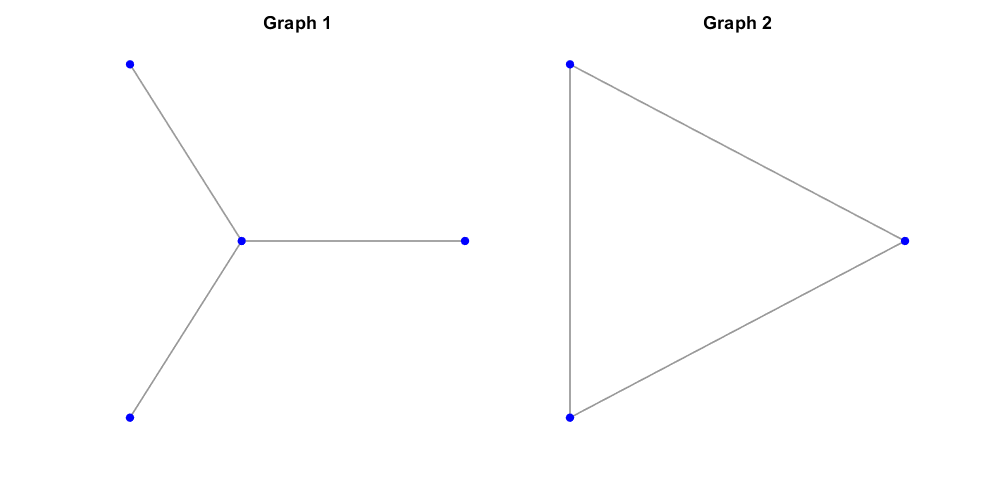
\includegraphics[width=0.45\textwidth]{gr1.png}\label{fig:gr1}}
        \hfill
        \subfloat[Graph 2]{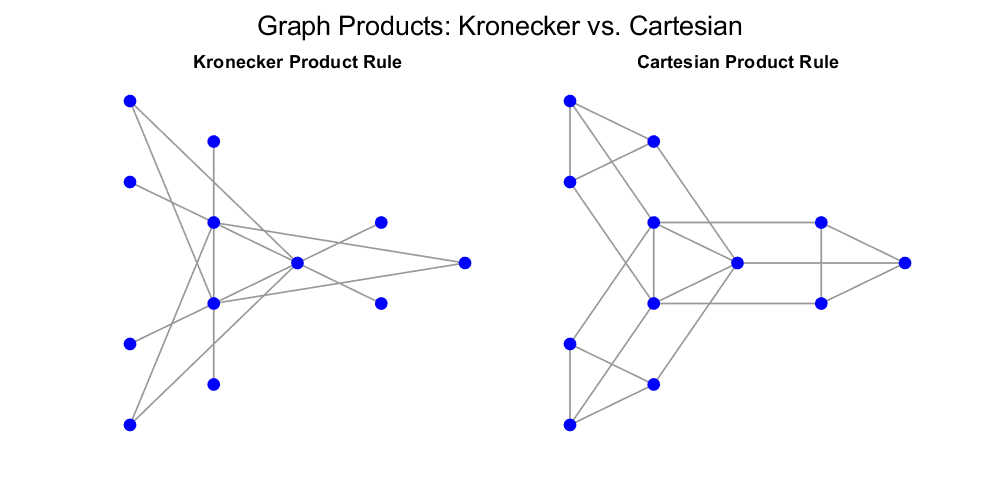
\includegraphics[width=0.45\textwidth]{gr2.png}\label{fig:gr2}}
        \caption{Graphs $G_1 , G_2$ with their Kronicker product $G_t$(left) and their Cartesian product $G_s$ (right) }
        \label{fig:graphs}
    \end{figure}
    
    \begin{lstlisting}
    w1 = [0, 0.7, 1.1, 2.3];    W1 = zeros(4);
    W1(1, :) = w1;              W1 = W1 + W1';
    G1 = gsp_comet(4, 3);   % Defining G1 ----------
    G1.W = W1;
    W2 = [0, 1.6, 2.4; 0, 0, 0.8; 0, 0, 0];    W2 = W2 + W2';
    G2 = gsp_ring(3);       % Defining G2 ----------
    G2.W = W2;
    pt.verbose = 1;
    pt.rule = 'kronecker';
    Gs = gsp_graph_product(G1, G2, pt);  % Defining Kronicker product
    pt.rule = 'cartesian';
    Gt = gsp_graph_product(G1, G2, pt);  % Defining Cartesian product
    \end{lstlisting}
    
    We know that for $G_t$ and $G_s$ the adjacency matrix are $A_t= A_1 \circledtimes A_2$ and $A_s = A_1 \circledtimes I_4 + I_3 \circledtimes A_2$, respectively. Where $A_1, A_2$ are the adjacency matrices for $G_1, G_2$, respectively. You can further investigate on the weight matrices for $G_t, G_s$ at 
    \texttt{Gt\_matrices.txt} and \texttt{Gs\_matrices.txt} on the results directory.
    
    % -------------------------------------------------------------
    \item In this section we chose $H=G_t$ and generated a random graph signal on $H$ and plotted the result using \texttt{gsp\_plot\_signal} on our graph which is depicted down below:

    %\clearpage

    \begin{figure}[h!]
        \centering
        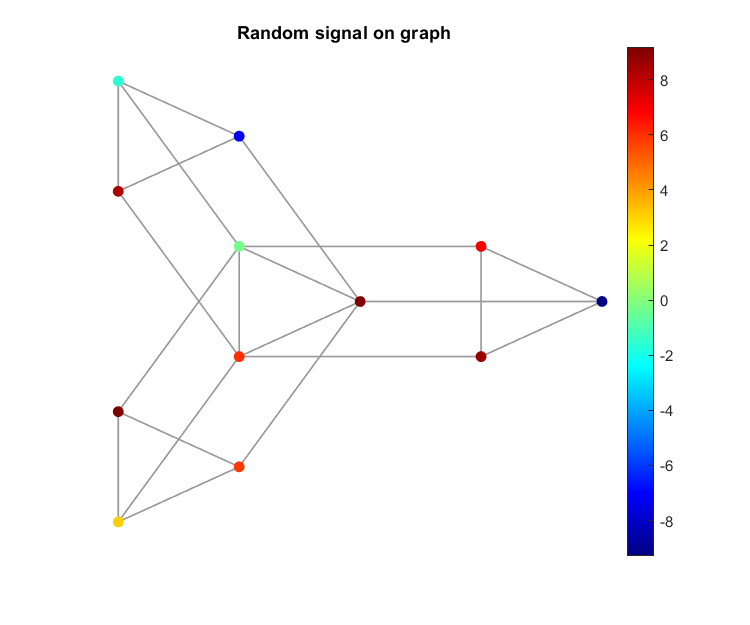
\includegraphics[scale=0.3]{gr3.png} % Resizing the image to half its size
        \caption{A random signal $x_H$ plotted with its associated graph $H$}
        \label{fig:gr3}
    \end{figure}

    \begin{lstlisting}
    H = Gt;
    x = rand(size(H.A, 1), 1) * 20 - 10;
    % Plotting the signal
    figure('Position', [100, 100, 600, 500]);
    title('Random signal on graph')
    gsp_plot_signal(H, x)
    \end{lstlisting}
    
     % -------------------------------------------------------------
    \item Now we will get the eigenvalues and eigenvectors of the Laplacian matrix of graph $H$, and show its spectrum using \texttt{gsp\_compute\_fourier\_basis} and \texttt{gsp\_gft}.

    \begin{figure}[h!]
        \centering
        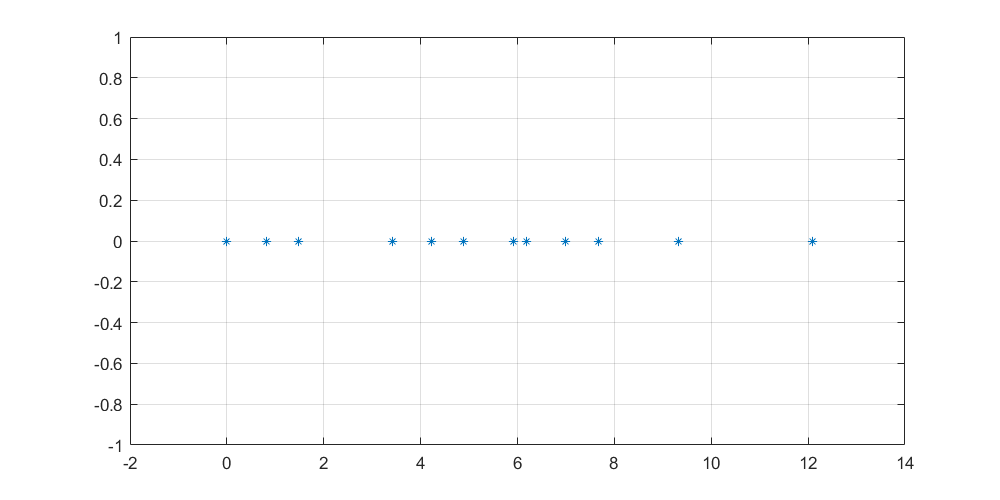
\includegraphics[scale=0.3]{gr4.png} % Resizing the image to half its size
        \caption{The spectrum of the graph $\{\lambda_1, ...,\lambda_n\}$}
        \label{fig:gr4}
    \end{figure}        
    Note that since the Laplacian matrix $L_H$ is symmetric, the eigenvalues of $L_H$ are real-valued.
    \\
    We can also show the random signal $x_H$ in part C, to show the spectrum of $X_H$ over the eigenvalues that we got:

    \clearpage
    
    \begin{figure}[h!]
        \centering
        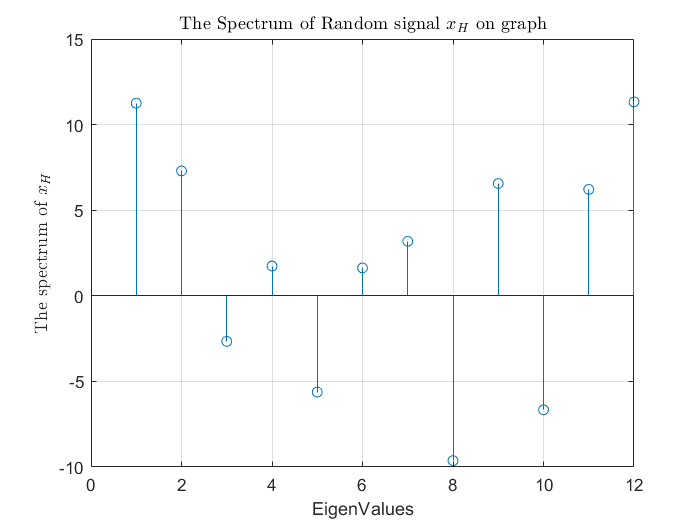
\includegraphics[scale=0.3]{gr6.png} % Resizing the image to half its size
        \caption{The spectrum of the random graph signal $x_H$ over $\{\lambda_1, ...,\lambda_n\}$}
        \label{fig:gr6}
    \end{figure} 

    \begin{lstlisting}
    H  = gsp_compute_fourier_basis(H);% computing the fourier basis of graph H
    spectrum = H.e;               % getting the eigenvalues(spectrum basis)
    x_hat = gsp_gft(H, x);        % computing the spectrum of x
    
    \end{lstlisting}

    
    % -------------------------------------------------------------
    \item Next, we will obtain the four eigenvectors corresponding to the two largest and two smallest eigenvalues. These eigenvalues will then be plotted as signals on the graph. The desired plot is shown below:

    %\clearpage

    \begin{figure}[h!]
        \centering
        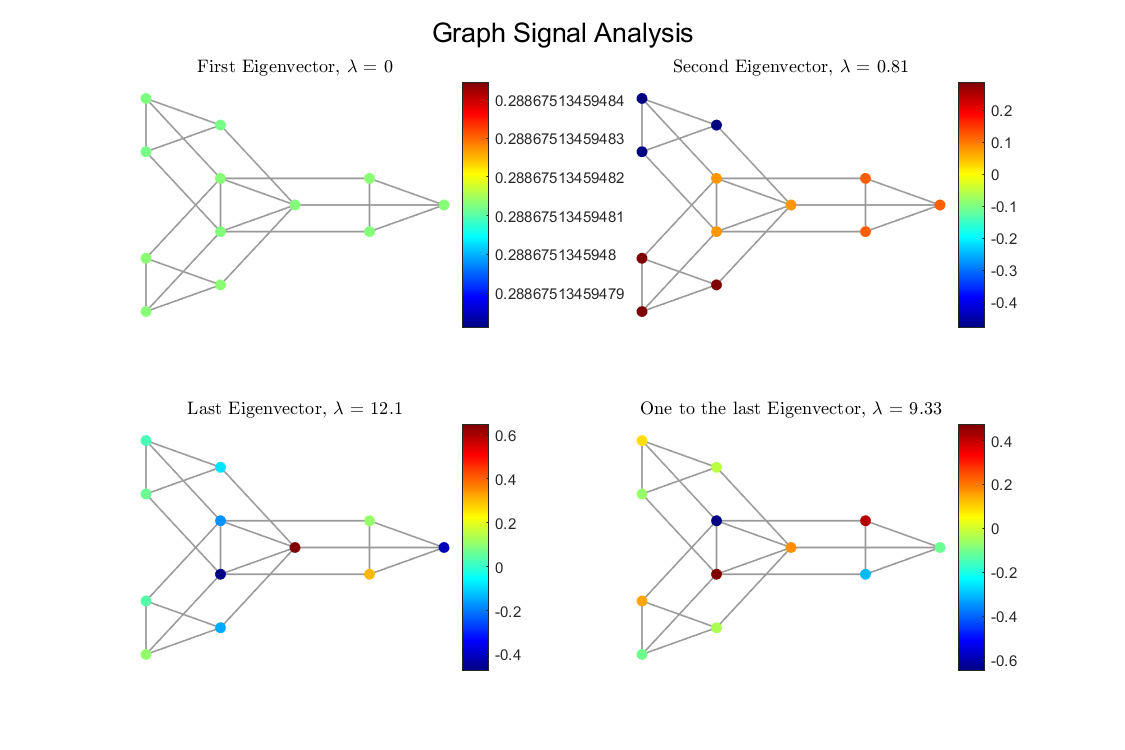
\includegraphics[scale=0.4]{gr5.png} % Resizing the image to half its size
        \caption{The spectrum of the random graph signal $x_H$ over $\{\lambda_1, ...,\lambda_n\}$}
        \label{fig:gr5}
    \end{figure} 

    As you can see, The signal with the least eigenvalue(which is zero) is smooth, and as the eigenvalues increases, the graph gets more and more non-smooth. As the eigenvector correspondent to eigenvalue $12.1=\lambda_{max}$ is of the most non-smoothness.
\end{enumerate}
% -------------------------------------------------------------
\maketitle
\section*{Problem 2}
\begin{enumerate}
    \item In this context we have a Stochastic Block Matrix $SBM(n,p,q)$ where we have two communities where each person is friend with its own community with the probability $p$ and is friend with the other community with the probability $q$.
    Thus, the expected value of the adjacency matrix over the distributions would be:

    \[
    \mathbb{E } [A] + p I_{n\times  n} = 
    \begin{bmatrix}
    \begin{array}{ccc|ccc}
    p & \cdots & p & q & \cdots & q \\
    \vdots & \ddots & \vdots & \vdots & \ddots & \vdots \\
    p & \cdots & p & q & \cdots & q \\
    \hline
    q & \cdots & q & p & \cdots & p \\
    \vdots & \ddots & \vdots & \vdots & \ddots & \vdots \\
    q & \cdots & q & p & \cdots & p \\
    \end{array}
    \end{bmatrix}
    \]
    Here is the implementation code of defining our SBM graph:
    
    \begin{lstlisting}
    % SBM params
    N = 1000;     p = 0.5;     q = 0.2;
    % Generate SBM graph
    dim = 2;     seed = 99;     rng(seed)
    sig = randi([0, dim - 1], [N, 1]);
    sig = 2 * rescale(sig) - 1;        % sig \in {+1,-1}
    P = (sig == sig') * p + (sig ~= sig') * q;
    A = ones(N) - (rand(N) > P);
    A = triu(A);
    A = abs(A - A');    % --- the Adjancency Matrix 
    % Create graph and compute Fourier basis
    G = gsp_graph(A);
    G = gsp_create_laplacian(G, 'normalized');
    G.type = 'normalized'; % or we could use unnormalized version
    G = gsp_compute_fourier_basis(G);
    \end{lstlisting}
    
    We know that the $(u_1, \lambda_1) = (\mathbb{1}_n, 0)$ is a pair of eigenvector, eigenvalues of the Laplacian matrix. So we would get the eigenvalues of the second least eigenvalues(if they are nonzero, otherwise we  would switch to bigger ones)
    and place each node $j$ with a point in 2 dimensional grid as $(u_2 (j), u_3 (j))$. And the key point is that the sign of the first coordinate of points(nodes) which is $(u_2 (j)$ will tell us to which community each node belongs. It is as if that our rule would be:

    \[
    \hat{\sigma_j} =
    \begin{cases} 
       +1, & \text{if } u_2 (j) \geq 0 \\
       -1, & \text{if } u_2 (j) < 0 \\
    \end{cases}
    \]
    Here, we used both Normalized Laplacian(the right image) and Unnormalized Laplacian(the left image) matrices. And this is the code and the final result of community detection:

    \begin{lstlisting}
    G = gsp_graph(A);
    % Use 'combinatorial' for unnormalized Laplacian
    G = gsp_create_laplacian(G, 'combinatorial'); 
    G.type = 'combinatorial';
    G = gsp_compute_fourier_basis(G);
    
    % Getting Fourier basis for visualization
    U23 = G.U;
    G.coords = U23(:, 2:max(3, dim));
    % Plotting parameters
    param = struct;
    param.colorbar = 0;
    G.plotting.edge_width = 0.1;
    figure;
    gsp_plot_signal(G, sig, param)
    title('SBM Graph Clustering - with Unnormalized Laplacian');
    \end{lstlisting}
    
    \clearpage

    \begin{figure}[h!]
        \centering
        \subfloat[Graph 1]{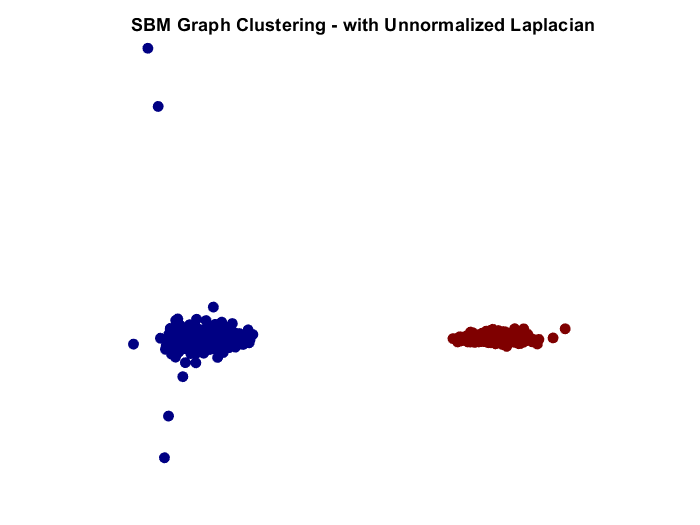
\includegraphics[width=0.45\textwidth]{gr7.png}\label{fig:gr8}}
        \hfill
        \subfloat[Graph 2]{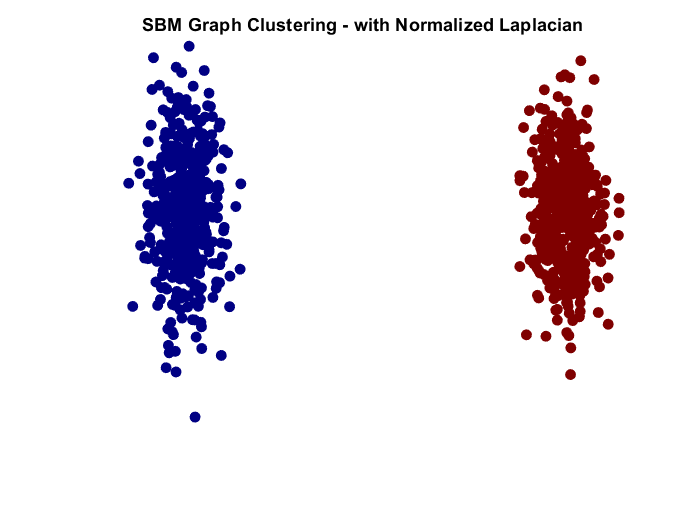
\includegraphics[width=0.45\textwidth]{gr8.png}\label{fig:gr8}}
        \caption{$SBM(n=1000,p=0.5,q=0.2)$ classification with the eigenvalues of Unnormalized and Normalized Laplacian Matrix of the graph }
        \label{fig:graphs}
    \end{figure}
    Furthermore, the task of classification with Normalized Laplacian Matrix seems
    better than the Unormalized Laplacian Matrix.
%-----------------------------------------------------------------
    \item First of all, the reason behind $p,q = \Theta(\frac{\log n}{n})$ is that if $p$ or $q$ is of $o(\frac{\log n}{n})$, then it would be a sparse graph and we wouldn't allow that. 
    \\ 
    On the other hand, as the distance between $p$ and $q$ rises, the classification gets harder, therefore we plot the ratio of true labeling(accuracy) versus a measure of $|\sqrt{\alpha}-\sqrt{\beta}|$. Here is the code and the result for plotting the accuracy.
\end{enumerate}

    \begin{figure}[h!]
        \centering
        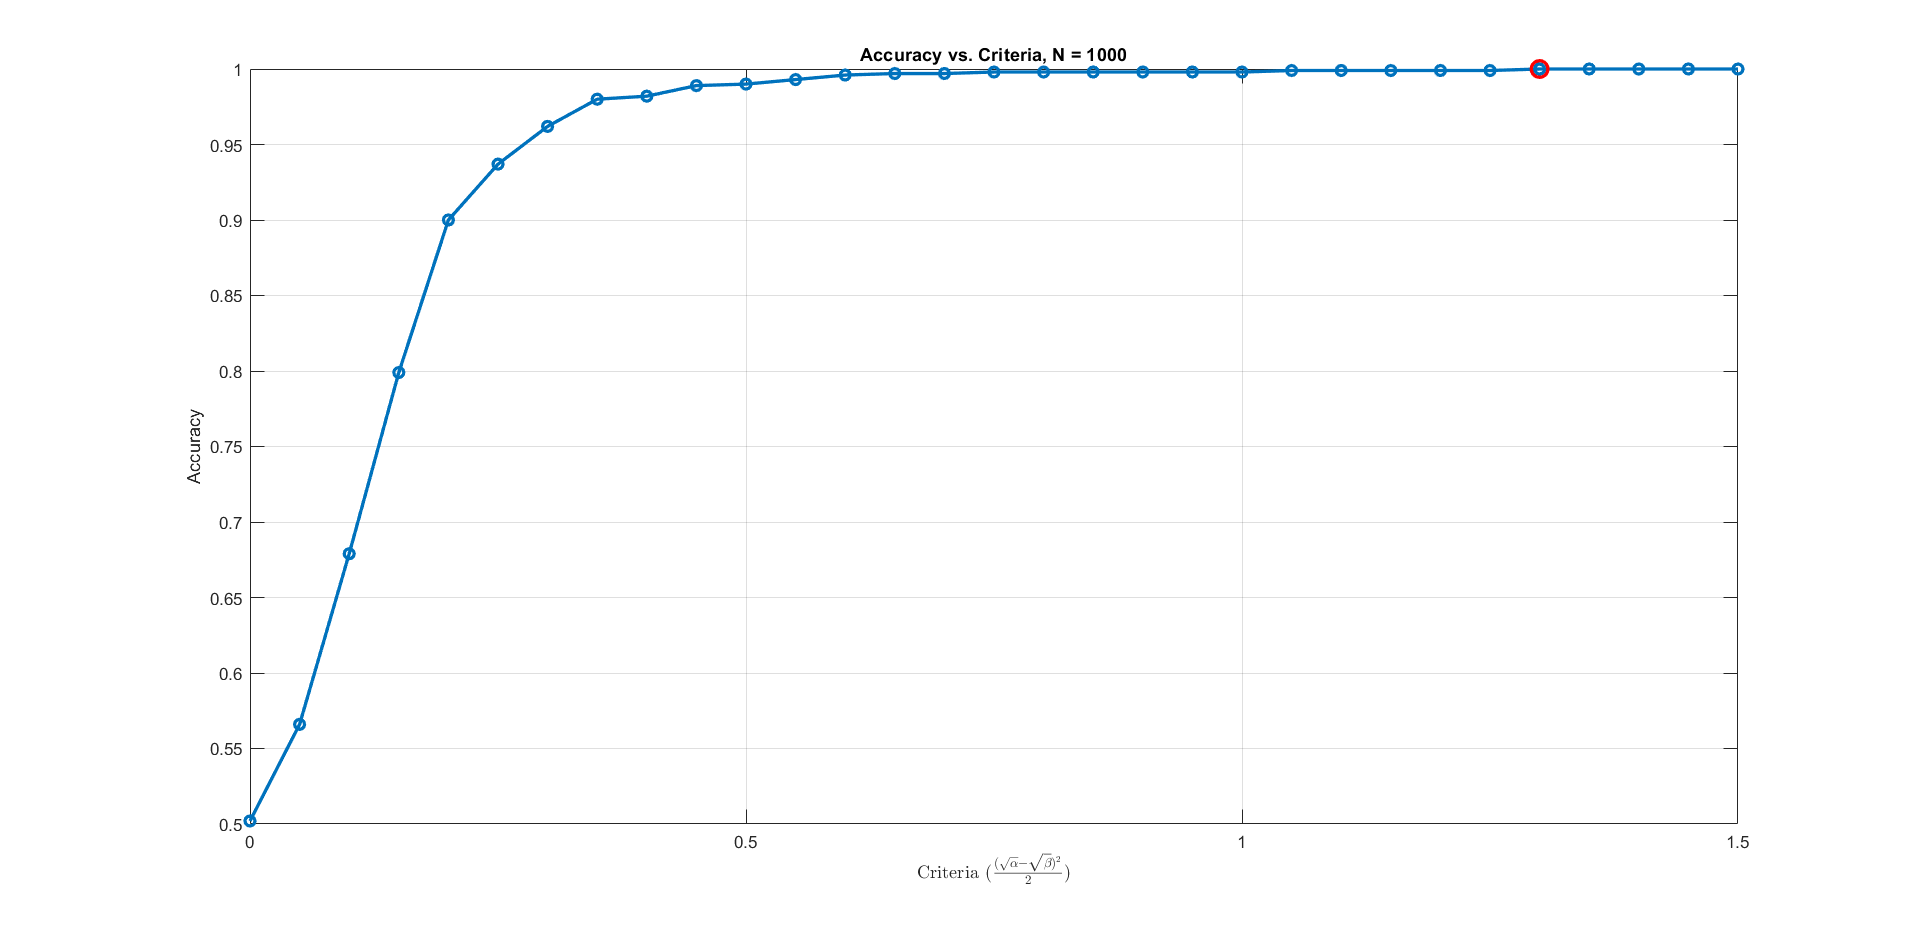
\includegraphics[scale=0.4]{gr9.png} % Resizing the image to half its size
        \caption{The accuracy versus criteria $|\sqrt{\alpha}-\sqrt{\beta}|^2$}
        \label{fig:gr9}
    \end{figure} 




\begin{lstlisting}
% Parameters of SBM
N = 1000;
seed = 99;
dim = 2;

% Sets of alpha and beta
criteria = 0:0.05:1.5;
alphas = 4 * ones(1, numel(criteria));
betas = (sqrt(alphas) - sqrt(2*criteria)).^2;

% Initialize arrays to store results
acc = zeros(1, numel(criteria));

disp('Simulation start')

% Loop through sets
for i = 1:numel(alphas)
    alpha = alphas(i);
    beta = betas(i);
    
    % Generate SBM graph
    p = alpha * log(N) / N;
    q = beta * log(N) / N;

    % Run clustering and store accuracy
    acc(i) = run_clustering(N, p, q, dim, seed);
end

disp('Simulation finished')

% Find the point where accuracy becomes 1 after a certain criterion
criterion_threshold = 1;
idx_threshold = find(acc == 1, 1, 'first');

% Plot accuracy vs. criteria
figure;
plot(criteria, acc, '-o', 'LineWidth', 2);
hold on;
plot(criteria(idx_threshold), 1, 'ro', 'MarkerSize', 10, 'LineWidth', 2);
hold off;
xlabel('Criteria (\(\frac{(\sqrt{\alpha} - \sqrt{\beta})^2}{2}\))', 'Interpreter', 'latex');
ylabel('Accuracy');
title(['Accuracy vs. Criteria, N = ' num2str(N)]);
grid on;


% Display threshold information
disp(['Criterion threshold for N = ' num2str(N) ': ' num2str(criteria(idx_threshold))]);

function acc = run_clustering(N, p, q, dim, seed)
    % Generate SBM graph
    rng(seed)
    sig = randi([0, dim - 1], [N, 1]);
    sig = 2 * rescale(sig) - 1;
    P = (sig == sig') * p + (sig ~= sig') * q;
    A = ones(N) - (rand(N) > P);
    A = triu(A);
    A = abs(A - A');

    % Create graph and compute Fourier basis
    G = gsp_graph(A);
    G = gsp_create_laplacian(G, 'normalized');
    G.type = 'normalized';
    G = gsp_compute_fourier_basis(G);

    % Choose subset of Fourier basis for visualization
    U23 = G.U;
    dim = 2;
    G.coords = U23(:, 2:max(dim, 3));

    % Perform k-means clustering
    k = 2;
    [clusters, ~] = kmeans(G.coords, k);
    % clusters = G.coords(:,1) > 0;

    % True labels based on the sign of sig
    true_labels = (sig + 1) / 2 + 1;

    % Calculate accuracy
    accuracy = sum(clusters == true_labels) / numel(true_labels);
    accuracy = max(accuracy, 1 - accuracy);

    % Display results
    alpha = p * N / log(N);
    beta = q * N / log(N);
    c = (sqrt(alpha) - sqrt(beta)) ^ 2 / 2;
    disp(['alpha = ' num2str(alpha) ', beta = ' num2str(beta) ...
        ', criteria = ' num2str(c) ', Accuracy: ' num2str(accuracy)]);

    acc = accuracy;
    
end
\end{lstlisting}
% --------------------------------------------------
\end{document}
